\documentclass{beamer}

\mode<presentation> {
	% The Beamer class comes with a number of default slide themes
	% which change the colors and layouts of slides. Below this is a list
	% of all the themes, uncomment each in turn to see what they look like.
	
	%\usetheme{default}
	%\usetheme{AnnArbor}
	%\usetheme{Antibes}
	%\usetheme{Bergen}
	%\usetheme{Berkeley}
	%\usetheme{Berlin}
	%\usetheme{Boadilla}
	%\usetheme{CambridgeUS}
	%\usetheme{Copenhagen}
	%\usetheme{Darmstadt}
	%\usetheme{Dresden}
	%\usetheme{Frankfurt}
	%\usetheme{Goettingen}
	%\usetheme{Hannover}
	%\usetheme{Ilmenau}
	%\usetheme{JuanLesPins}
	%\usetheme{Luebeck}
	\usetheme{Madrid}
	%\usetheme{Malmoe}
	%\usetheme{Marburg}
	%\usetheme{Montpellier}
	%\usetheme{PaloAlto}
	%\usetheme{Pittsburgh}
	%\usetheme{Rochester}
	%\usetheme{Singapore}
	%\usetheme{Szeged}
	%\usetheme{Warsaw}
	
	% As well as themes, the Beamer class has a number of color themes
	% for any slide theme. Uncomment each of these in turn to see how it
	% changes the colors of your current slide theme.
	
	%\usecolortheme{albatross}
	\usecolortheme{beaver}
	%\usecolortheme{beetle}
	%\usecolortheme{crane}
	%\usecolortheme{dolphin}
	%\usecolortheme{dove}
	%\usecolortheme{fly}
	%\usecolortheme{lily}
	%\usecolortheme{orchid}
	%\usecolortheme{rose}
	%\usecolortheme{seagull}
	%\usecolortheme{seahorse}
	%\usecolortheme{whale}
	%\usecolortheme{wolverine}
	
	%\setbeamertemplate{footline} % To remove the footer line in all slides uncomment this line
	%\setbeamertemplate{footline}[page number] % To replace the footer line in all slides with a simple slide count uncomment this line
	
	%\setbeamertemplate{navigation symbols}{} % To remove the navigation symbols from the bottom of all slides uncomment this line
}
\usepackage[backend=biber]{biblatex}
\setbeamertemplate{caption}[numbered]
\newcommand{\btVFill}{\vskip0pt plus 1filll}
\usepackage{algorithm}
\usepackage{amsmath}
\usepackage{caption}
\usepackage{fec}
\usepackage{xcolor}
%----------------------------------------------------------------------------------------
%	TITLE PAGE
%----------------------------------------------------------------------------------------

\title[Warm Starting Series of MILP's]{Warm Starting Series of Mixed-Integer Linear Programs}
\author{Sean Kelley} % Your name
\date{22 September 2022} % Date, can be changed to a custom date

\AtBeginSection[]{
	\begin{frame}
		\vfill
		\centering
		\begin{beamercolorbox}[sep=8pt,center,shadow=true,rounded=true]{title}
			\usebeamerfont{title}\insertsectionhead\par%
		\end{beamercolorbox}
		\vfill
	\end{frame}
}

\begin{document}
	
	\begin{frame}
		\titlepage % Print the title page as the first slide
	\end{frame}

	\begin{frame}{Overview}
		\tableofcontents
	\end{frame}

	\section{Background}
	
	\begin{frame}[t]
		\frametitle{Motivation}
		\small
		\begin{itemize}
			\item Mixed-Integer Programming has created great value in industry.
			\item One important source comes from problems solved by a series of Mixed-Integer Linear Programs (MILPs).
			\begin{itemize}
				\item Electric Grid Production Planning (Stochastic Dual Decomposition)
				\item Vehicle Routing (Branch and Price)
			\end{itemize}
			\item Many MILP instances in such series differ only by objective coefficients or bounds on their constraints.
			\item Solvers can leverage what they discover solving one MILP to more quickly solve a similar MILP (a.k.a. "Warm Start").
			\item Warm starting would enable greater performance and expand the space of tractable problems for those solved as a series of MILPs.
		\end{itemize}
		\vspace{-.25cm}
		\begin{block}{}
			This presentation outlines a potential opportunity to warm start series of MILPs and discusses details towards its implementation.
		\end{block}
		\normalsize
	\end{frame}

	\begin{frame}[t]
		\frametitle{Simple Example}
		\footnotesize
		% what kind of information can a solver glean from a previous similar solve
		% two MILP's and their trees
		% Plug (2)'s bounds into (1)'s subproblems (get the right)
		% Gives us a branching decision (disjunction), primal solutions and dual bounds
		% Get similar tree by plugging in new objective instead of bounds
		\begin{columns}[T]
			\begin{column}{0.3\textwidth}
				\vspace{-.25cm}
				\begin{align}
					\begin{split}
						\text{max} \quad &x + 4y \\
						\text{s.t.} \; \; -&\frac{x}{2} + y \leq 2, \\
						&x + \frac{y}{2} \leq 4, \\
						(&x, y) \in \Zmbb^2_+
					\end{split}
					\label{left}
				\end{align}
				\begin{itemize}
					\item Solving (\ref{left}) yields Figure \ref{p:before}'s Branch and Bound tree.
					\item Constraints like "$x \leq 2$ or $x \geq 3$" cause branching.
					\item Such constraints are called \textbf{disjunctions}.
					\item We refer to their collection as \textit{the} disjunction.
				\end{itemize}
			\end{column}
			\begin{column}{0.7\textwidth}
				\vspace{-.25cm}
				\begin{figure}[h]
					\resizebox{.45\textwidth}{!}{%
						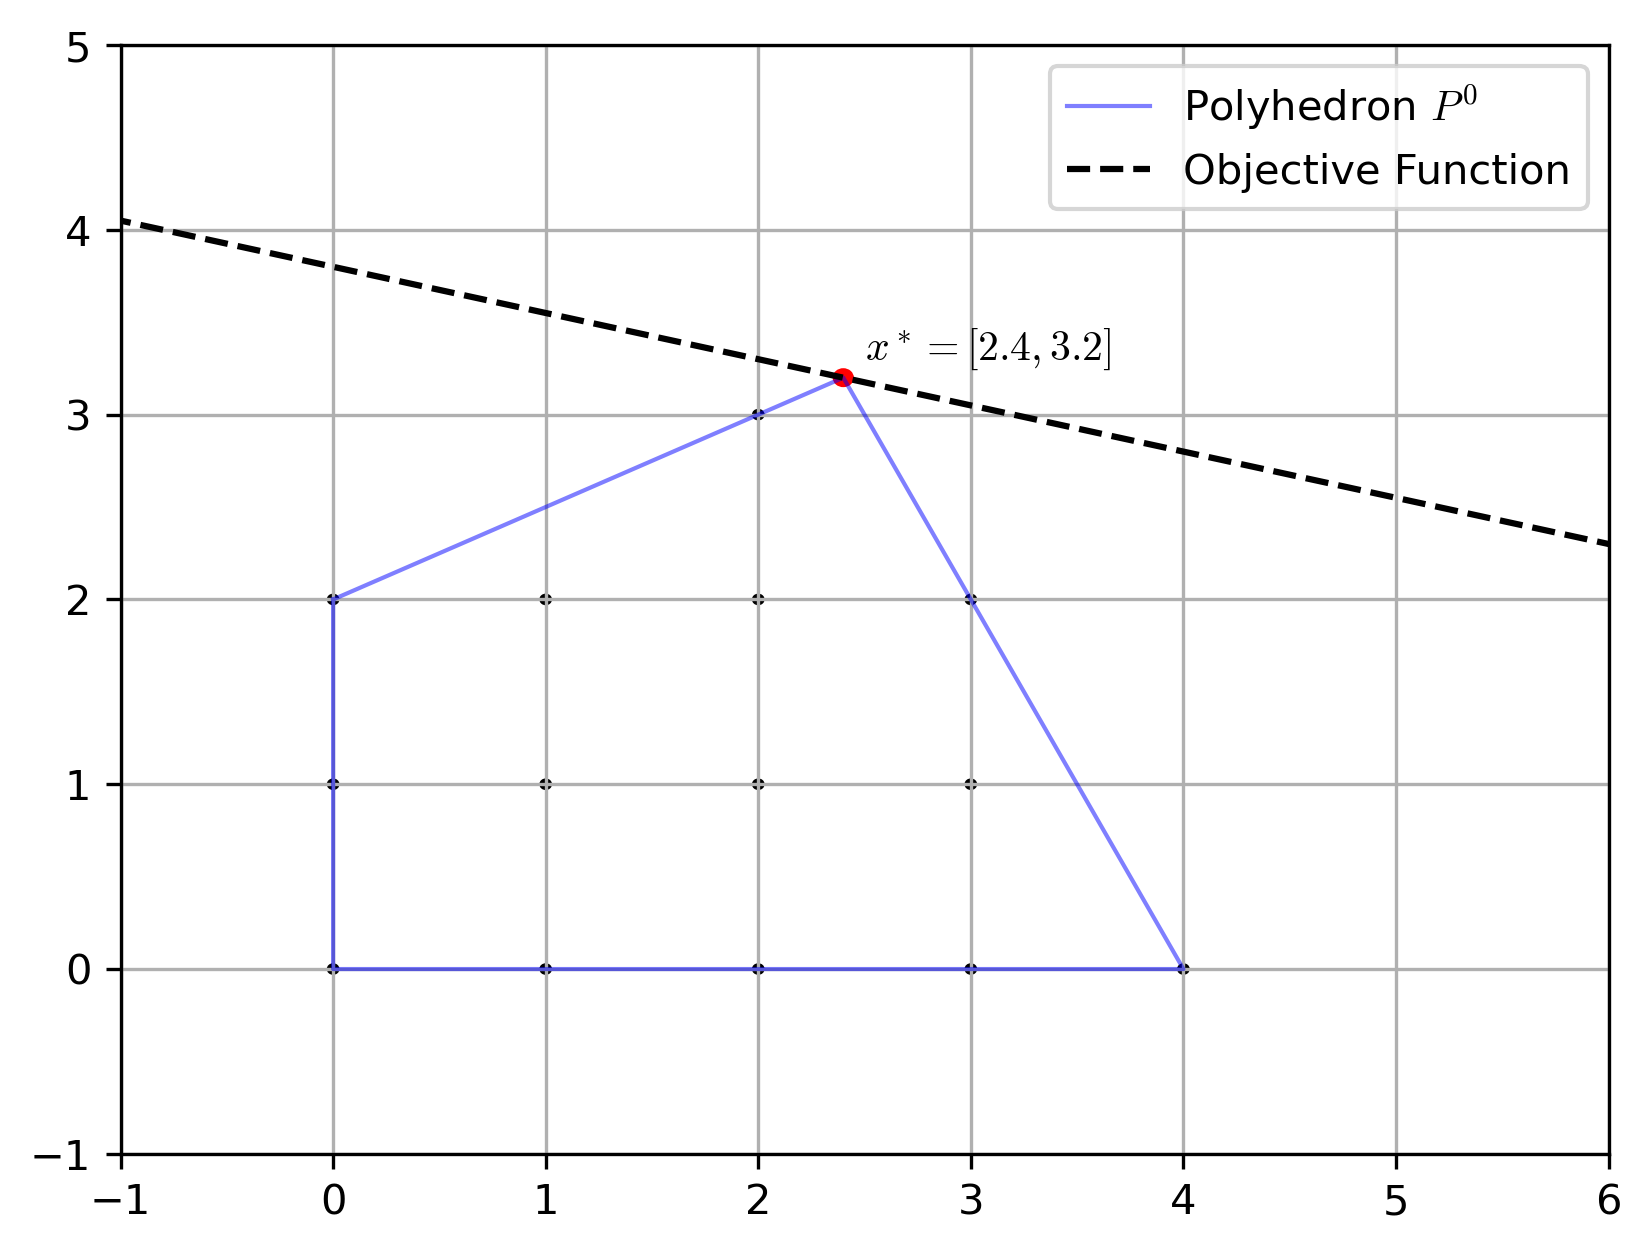
\includegraphics[]{P0.png}
					}
					% \caption{Node 0 LP relaxation}
					\label{p:root}
				\end{figure}
				\vspace{-.25cm}
				\centering
				Branch on $ x \leq 2 $ or $ x \geq 3 $
				\vspace{-.25cm}
				\begin{figure}[]
					\centering
					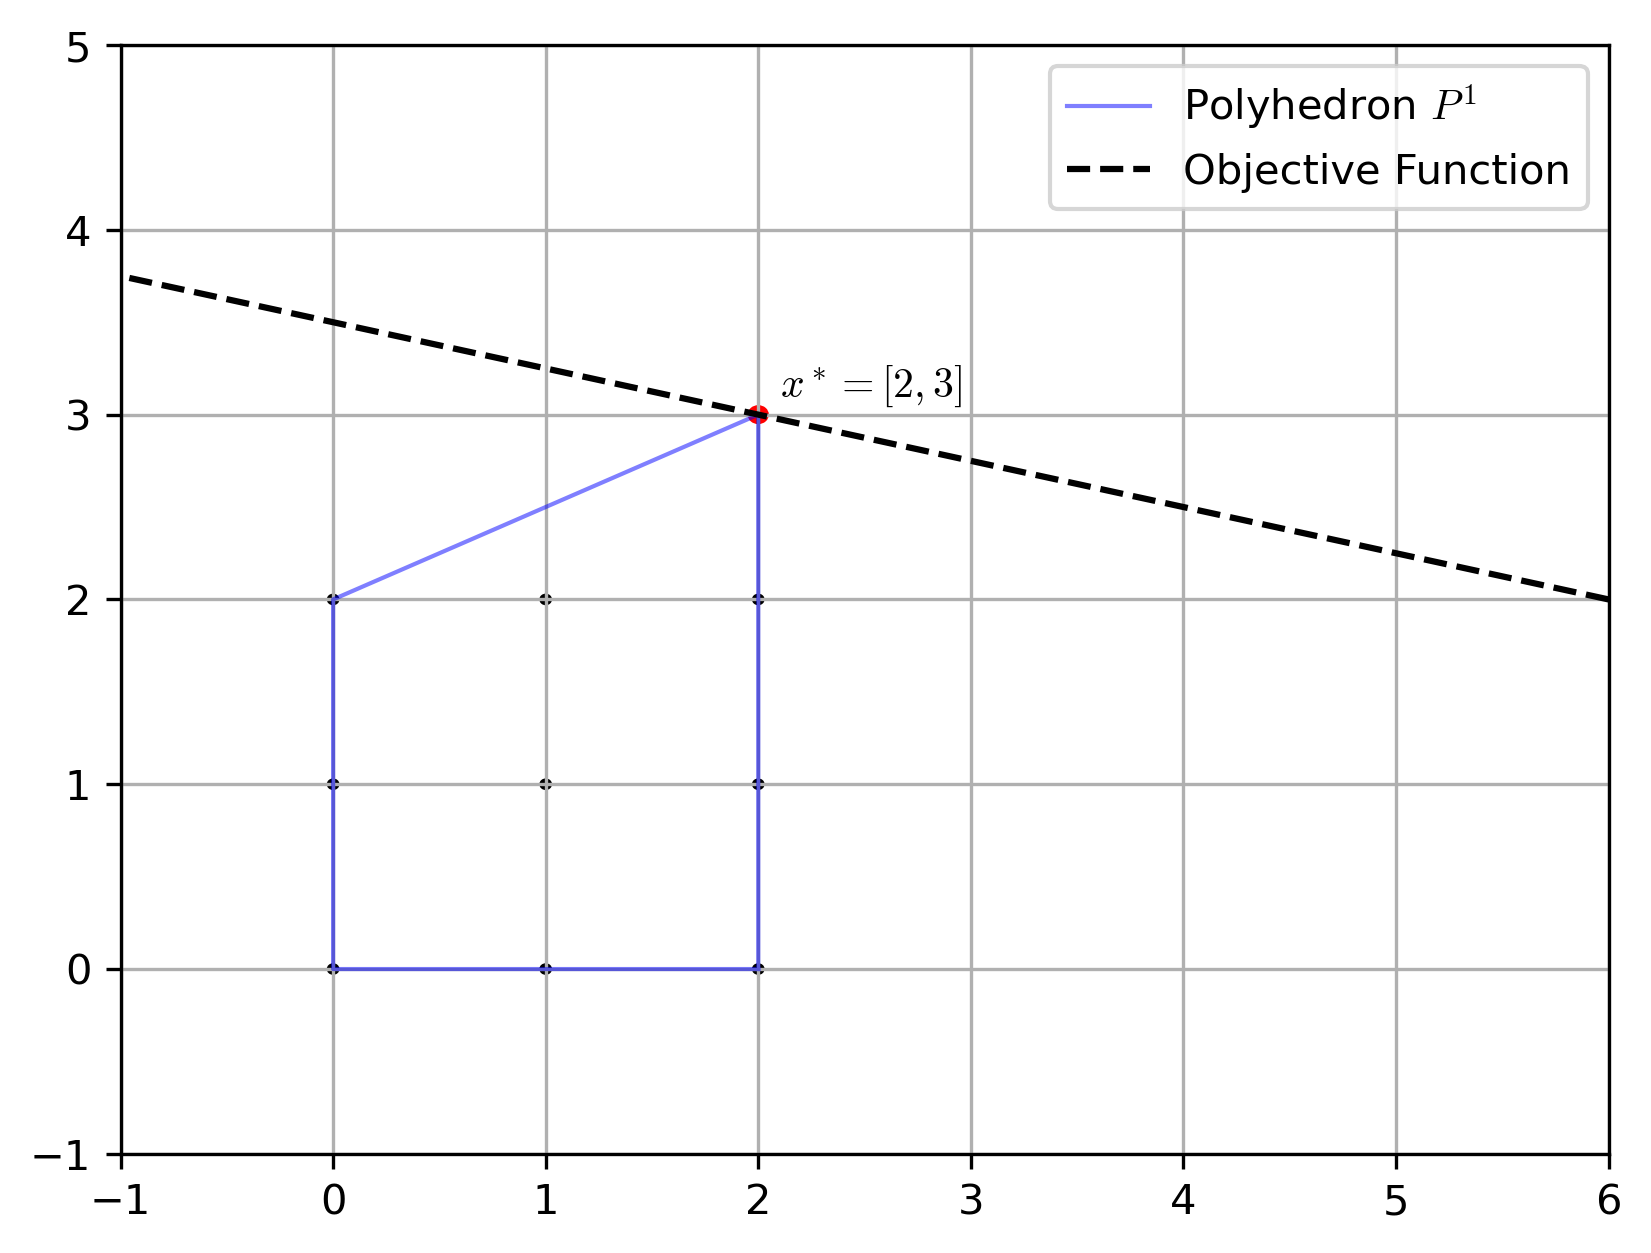
\includegraphics[width=.45\textwidth]{P1.png}
					\hfill
					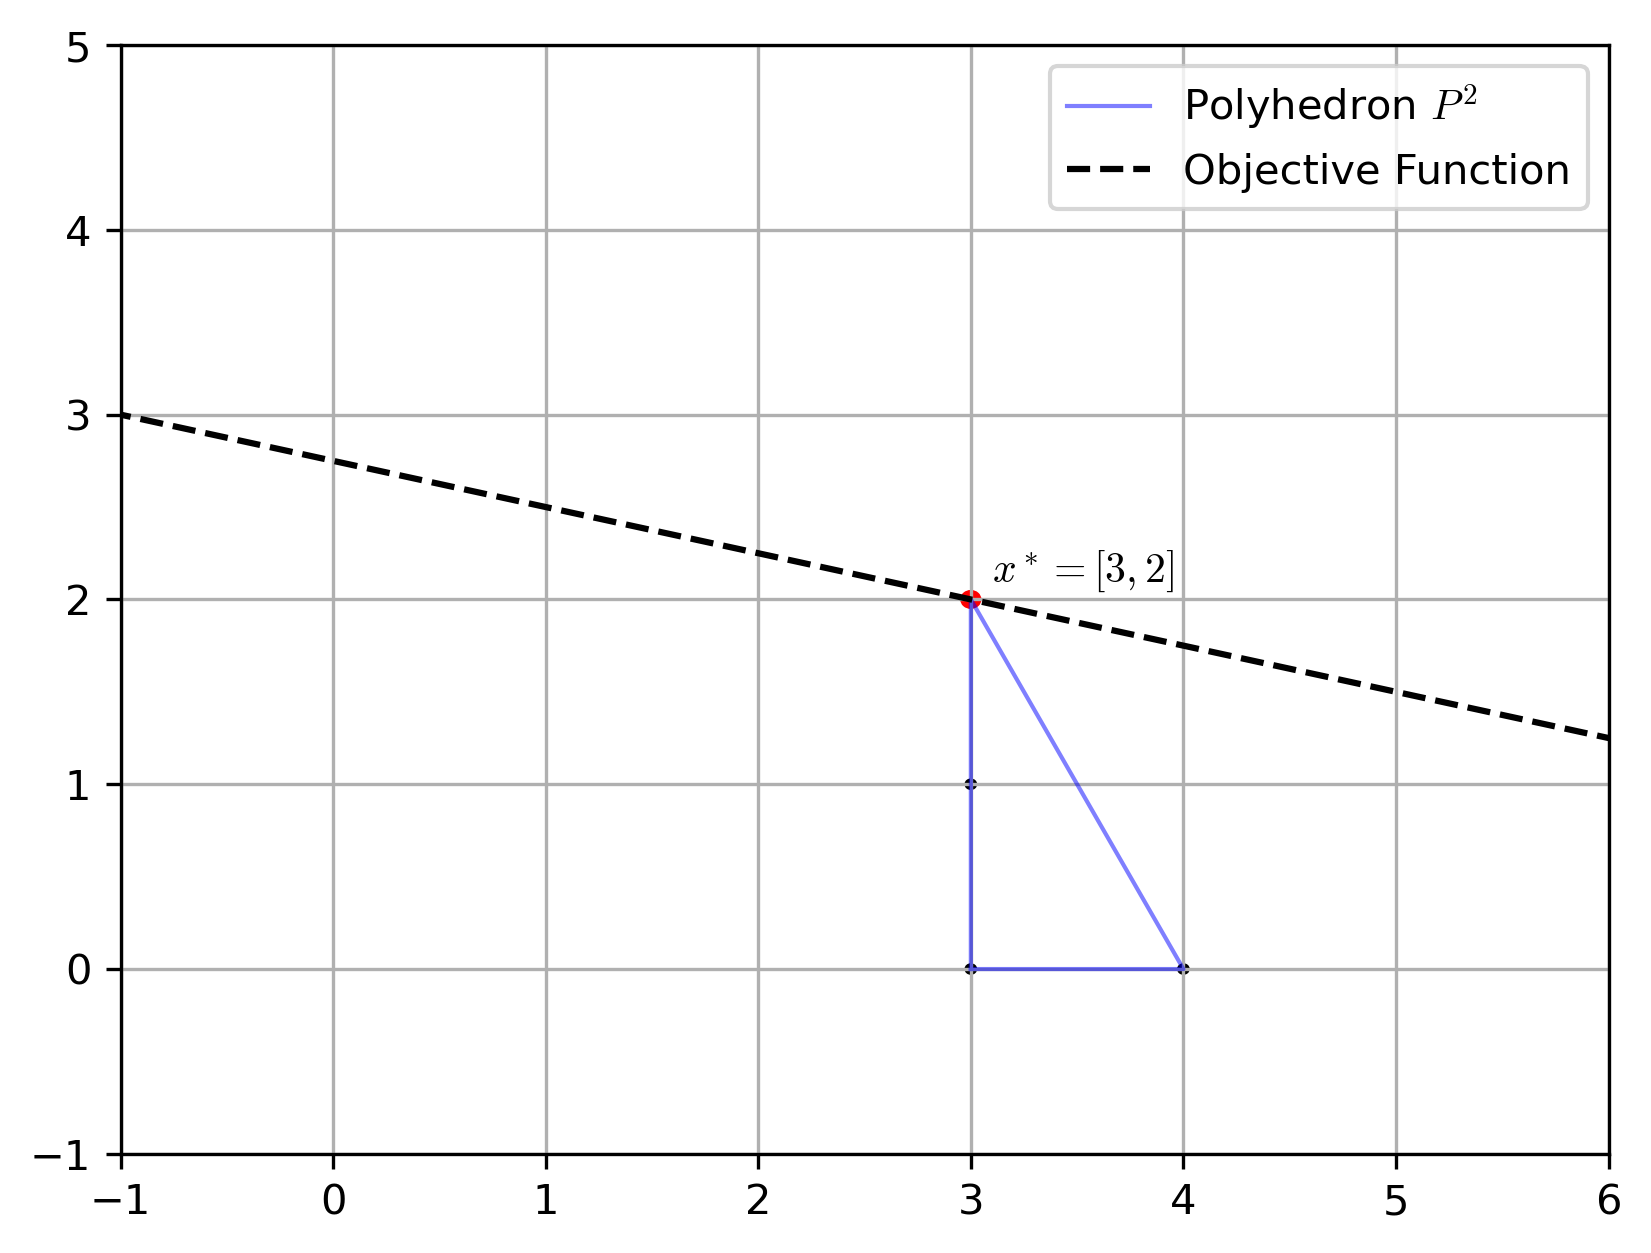
\includegraphics[width=.45\textwidth]{P2.png}
					\captionsetup{font=footnotesize,labelfont=footnotesize}
					\caption{(\ref{left})'s Branch and Bound tree}
					\label{p:before}
				\end{figure}
			\end{column}
		\end{columns}
		\normalsize
	\end{frame}

	\begin{frame}[t]
		\frametitle{Simple Example}
		\footnotesize
		% what kind of information can a solver glean from a previous similar solve
		% two MILP's and their trees
		% Plug (2)'s bounds into (1)'s subproblems (get the right)
		% Gives us a branching decision (disjunction), primal solutions and dual bounds
		% Get similar tree by plugging in new objective instead of bounds
		\begin{columns}[T]
			\begin{column}{0.3\textwidth}
				\vspace{-.25cm}
				\begin{align}
					\begin{split}
						\text{max} \quad &x + 4y \\
						\text{s.t.} \; \; -&\frac{x}{2} + y \leq 3, \\
						&x + \frac{y}{2} \leq 5, \\
						(&x, y) \in \Zmbb^2_+
					\end{split}
					\label{right}
				\end{align}
				\begin{itemize}
					\item (\ref{right}) loosens the RHS from (\ref{left}).
					\item Applying (\ref{left})'s disjunction yields a partial Branch and Bound tree for (\ref{right}).
					\item This partial tree immediately yields the solution for (\ref{right}).
				\end{itemize}
			\end{column}
			\begin{column}{0.7\textwidth}
				\vspace{3.25cm}
				\centering
				Branch on $ x \leq 2 $ or $ x \geq 3 $
				\vspace{-.25cm}
				\begin{figure}[]
					\centering
					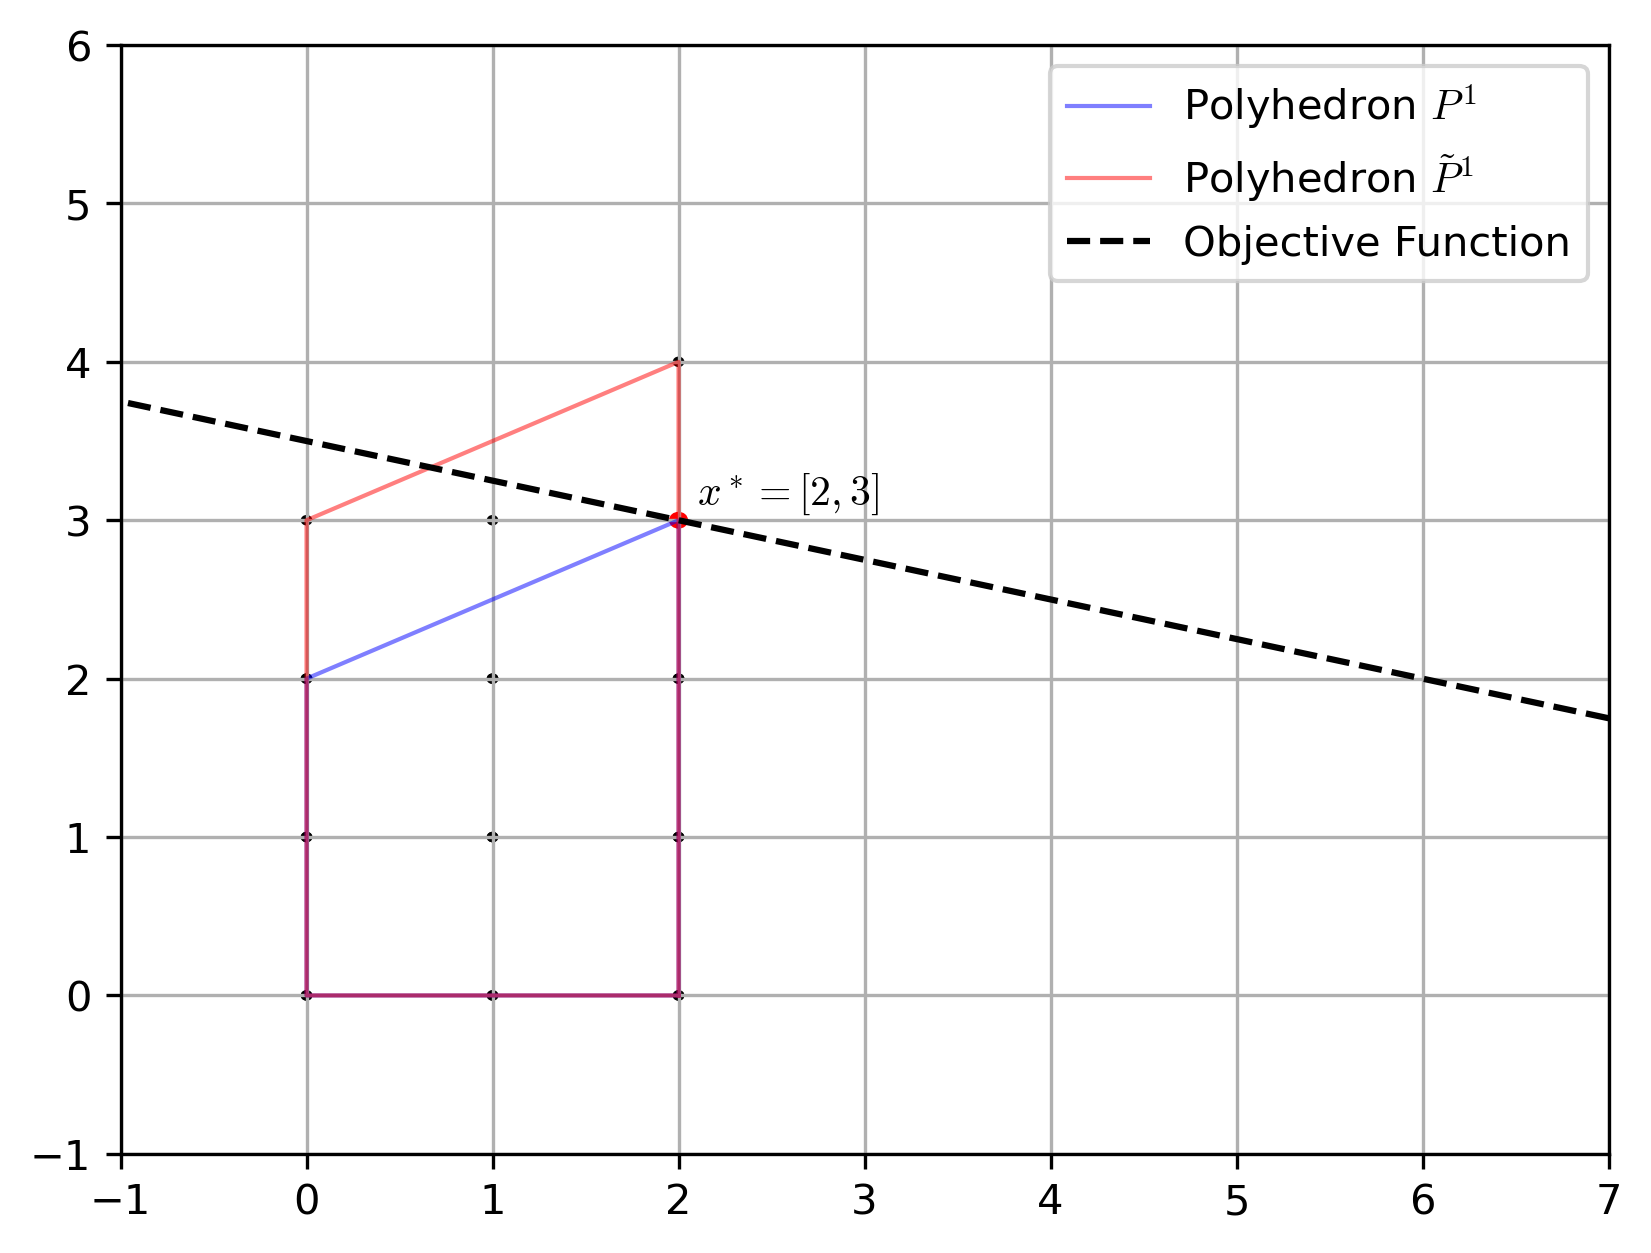
\includegraphics[width=.45\textwidth]{P1_prime.png}
					\hfill
					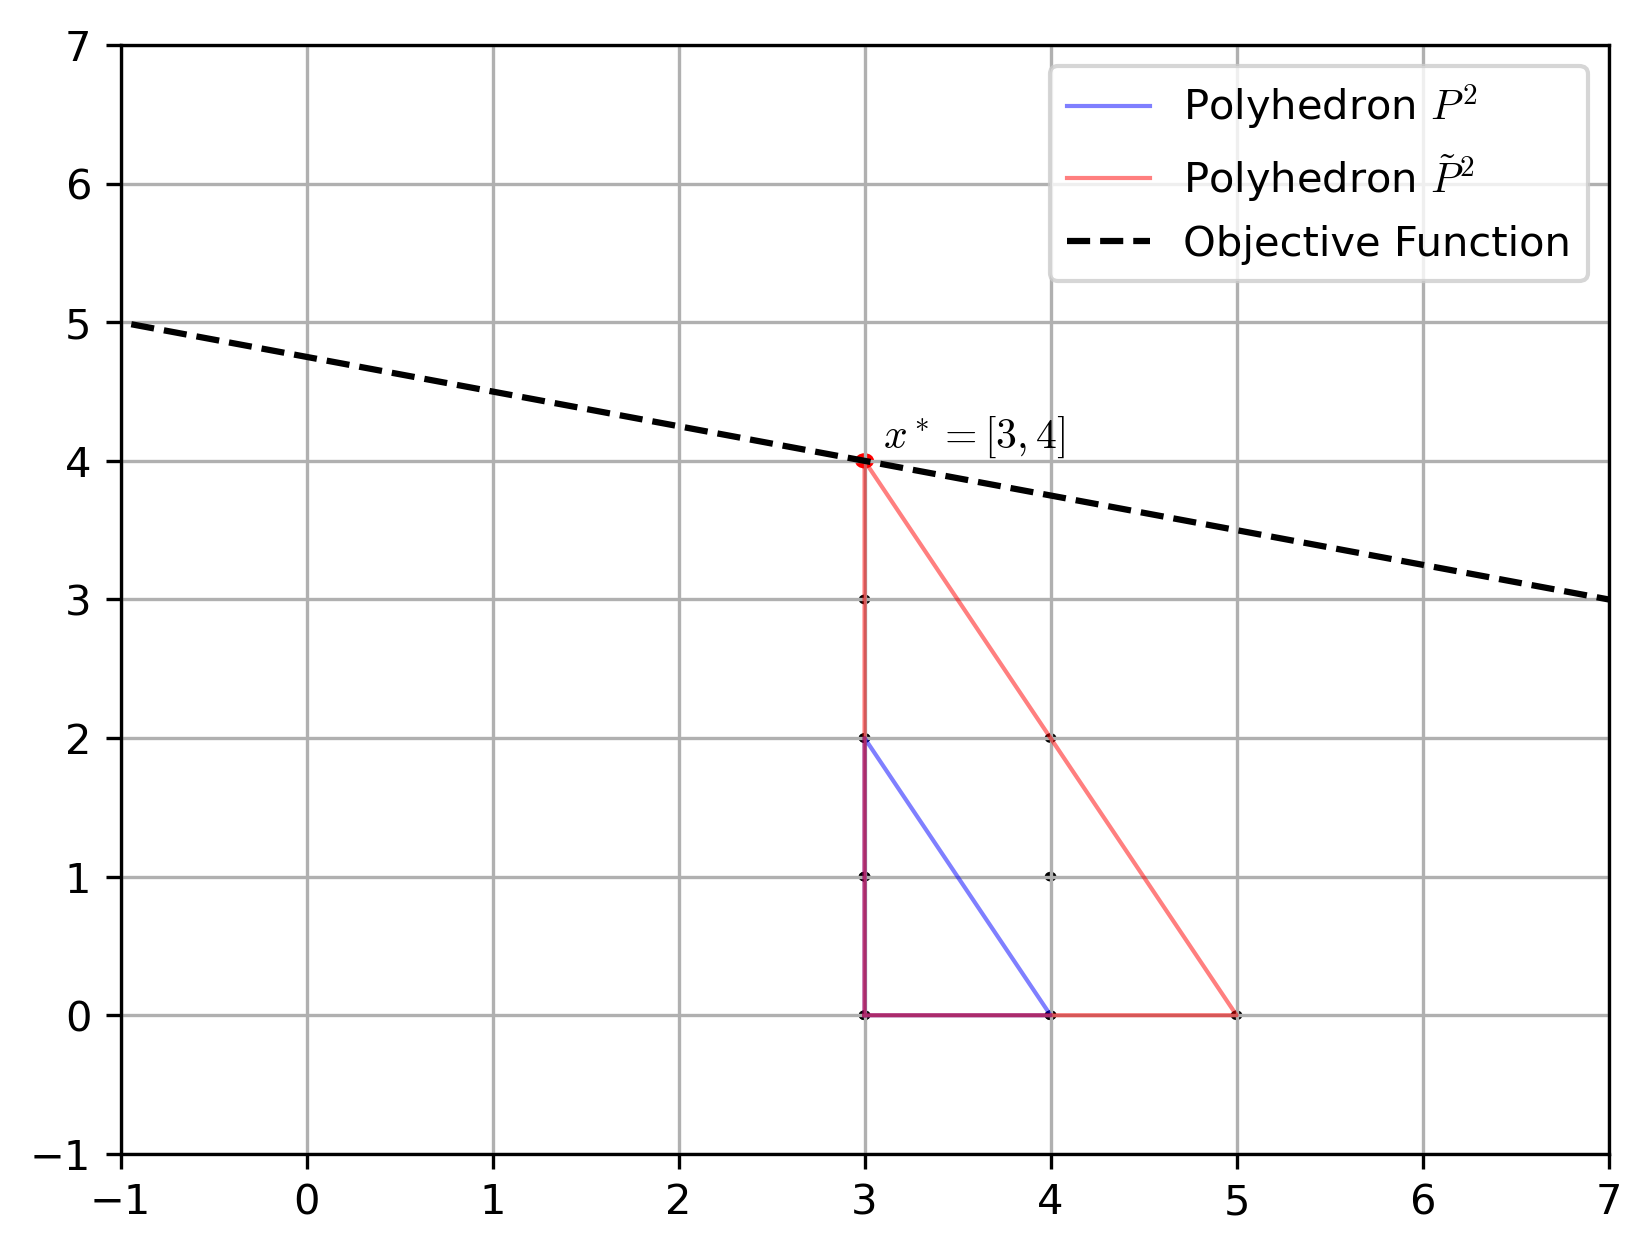
\includegraphics[width=.45\textwidth]{P2_prime.png}
					\captionsetup{font=footnotesize,labelfont=footnotesize}
					\caption{(\ref{right})'s partial Branch and Bound tree}
					\label{p:partial_after}
				\end{figure}
			\end{column}
		\end{columns}
		\normalsize
	\end{frame}

	\begin{frame}[t]
		\frametitle{Simple Example}
		\footnotesize
		% what kind of information can a solver glean from a previous similar solve
		% two MILP's and their trees
		% Plug (2)'s bounds into (1)'s subproblems (get the right)
		% Gives us a branching decision (disjunction), primal solutions and dual bounds
		% Get similar tree by plugging in new objective instead of bounds
		\begin{columns}[T]
			\begin{column}{0.3\textwidth}
				\begin{itemize}
					\item Solving (\ref{right}) yields Figure \ref{p:full_after}'s Branch and Bound tree.
					\item Figure \ref{p:full_after} contains the partial tree from Figure \ref{p:partial_after}.
					\item Applying Branch and Bound or the disjunction from (\ref{left}) both yield the same solution.
				\end{itemize}
			\end{column}
			\begin{column}{0.7\textwidth}
				\vspace{-.85cm}
				\begin{figure}[h]
					\resizebox{.45\textwidth}{!}{%
						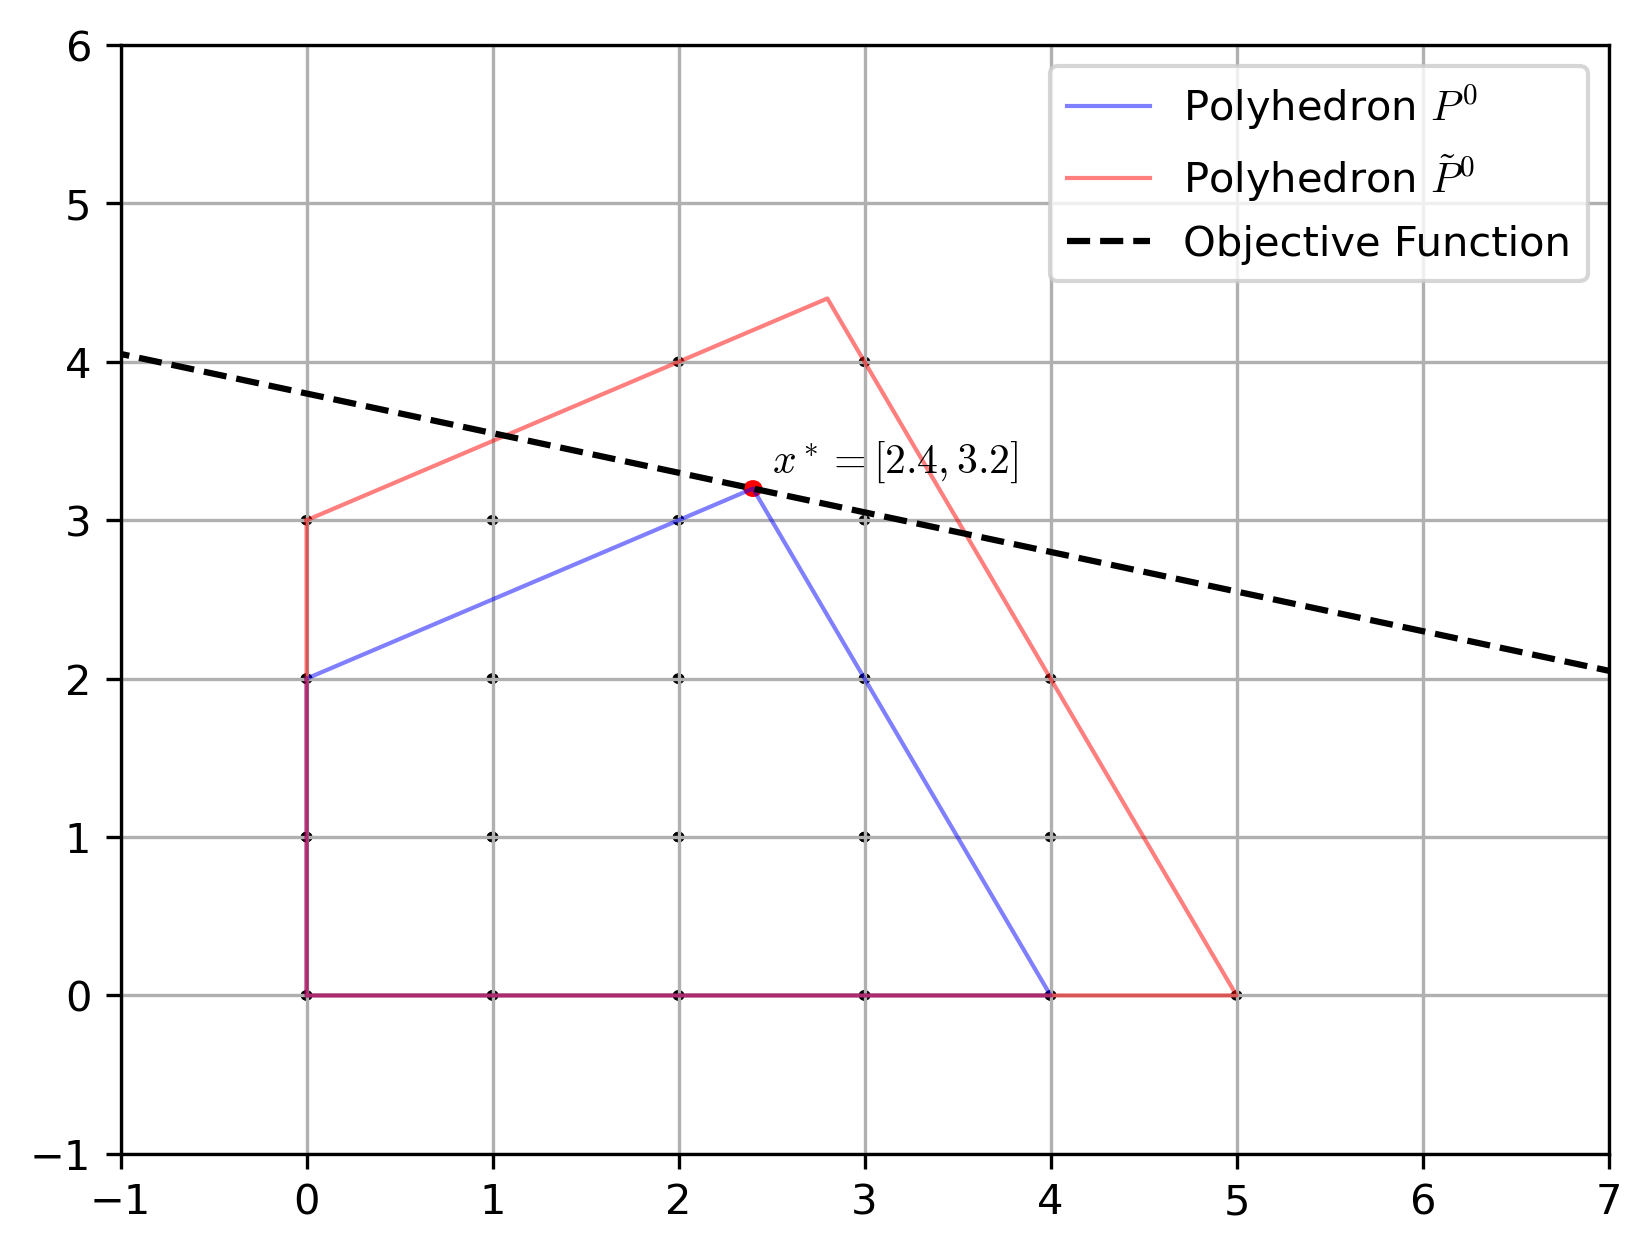
\includegraphics[]{P0_prime.png}
					}
					% \caption{Node 0 LP relaxation}
					\label{p:root_prime}
				\end{figure}
				\vspace{-.25cm}
				\centering
				Branch on $ x \leq 2 $ or $ x \geq 3 $
				\vspace{-.25cm}
				\begin{figure}[]
					\centering
					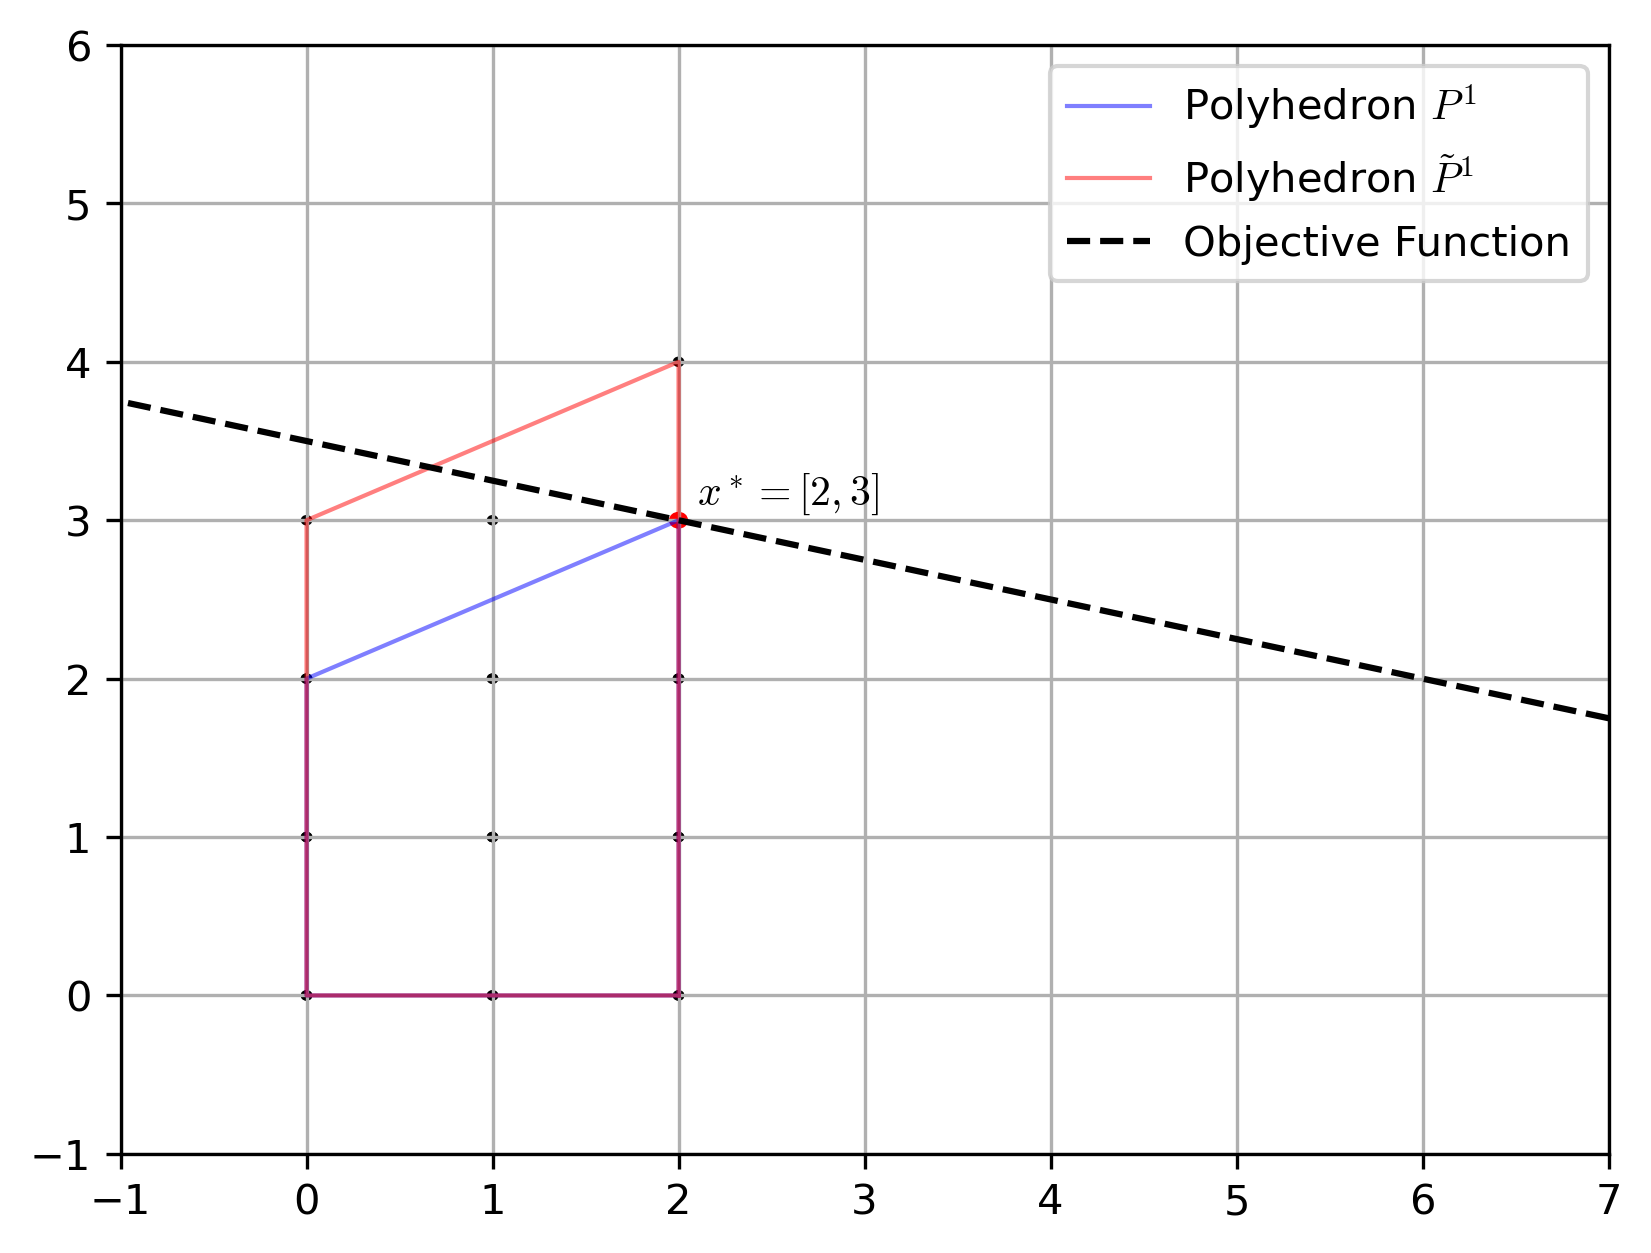
\includegraphics[width=.45\textwidth]{P1_prime.png}
					\hfill
					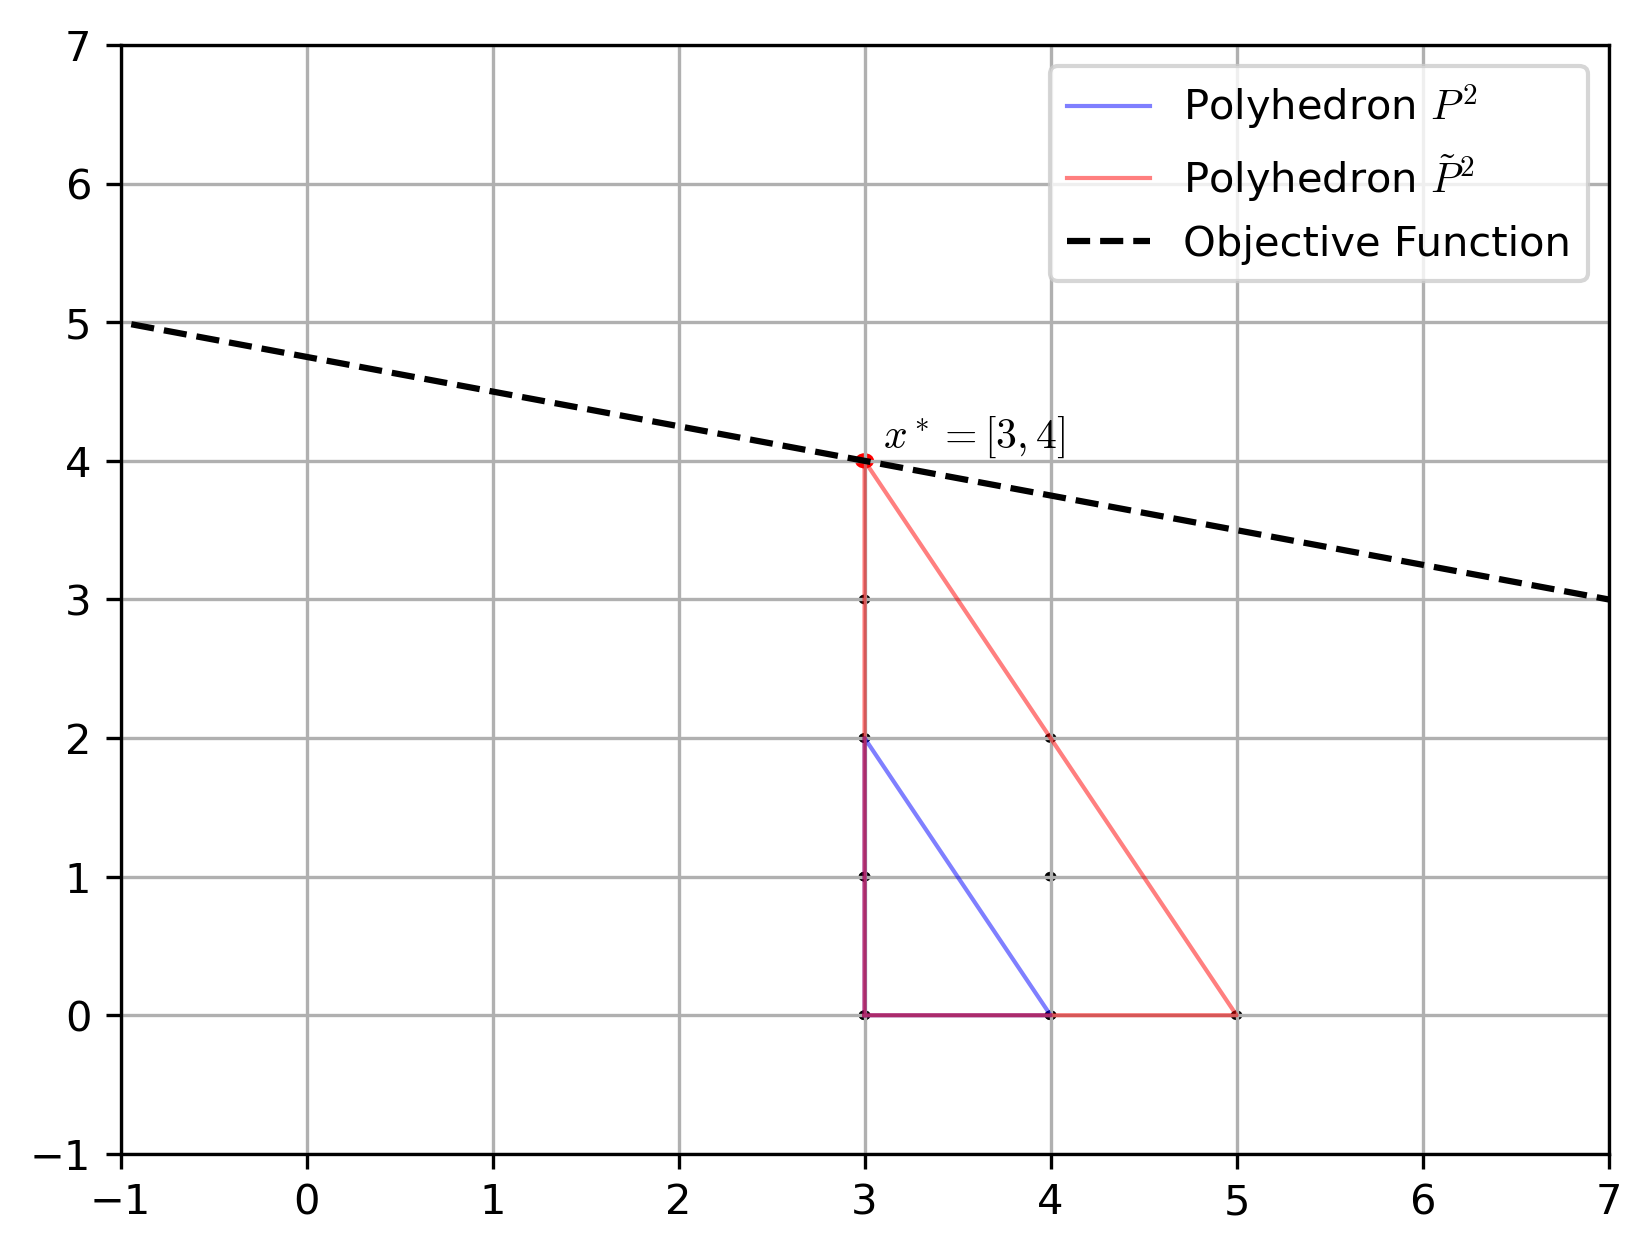
\includegraphics[width=.45\textwidth]{P2_prime.png}
					\captionsetup{font=footnotesize,labelfont=footnotesize}
					\caption{(\ref{right})'s full Branch and Bound tree}
					\label{p:full_after}
				\end{figure}
			\end{column}
		\end{columns}
		\vspace{-.35cm}
		\begin{block}{}
			Applying the disjunction from (\ref{left}) to (\ref{right}) is a warm start since it requires processing fewer nodes to find a solution than Branch and Bound alone.
		\end{block}
		\normalsize
	\end{frame}

	\begin{frame}[t]
		\frametitle{Generalizing}
		\small
		Consider the following two MILP's:
		\begin{columns}[T]
			\begin{column}{0.5\textwidth}
				\vspace{-.25cm}
				\begin{align}
					\begin{split}
						\text{min}& \qquad \quad c^T x \\
						\text{s.t.}& \; x \in P^0 \cap \Zmbb^p_+  \times \Rmbb^{n-p}_+ \\
					\end{split}
					\label{milp}
					\tag{MILP}
				\end{align}
				\; where
				\begin{align*}
					P^0 = \{x \in \Rmbb^n : Ax \geq b\} \qquad
				\end{align*}
			\end{column}
			\begin{column}{0.5\textwidth}
				\vspace{-.25cm}
				\begin{align}
					\begin{split}
						\text{min}& \qquad \quad \bar{c}^T x \\
						\text{s.t.}& \; x \in \bar{P}^0 \cap \Zmbb^p_+  \times \Rmbb^{n-p}_+ \\
					\end{split}
					\label{milpbar}
					\tag{$ \overline{\text{MILP}} $}
				\end{align}
				\vspace{.25cm}
				\begin{align*}
					\bar{P^0} = \{x \in \Rmbb^n : Ax \geq \bar{b}\} \qquad
				\end{align*}
			\end{column}
		\end{columns}
		\vspace{.25cm}
		We'll make the following assumptions about (\ref{milp}) and (\ref{milpbar}):
		\begin{itemize}
			\item Either $ c = \bar{c} $ or $ b = \bar{b} $.
			\item (\ref{milp}) has been solved with Branch and Bound.
			\item (\ref{milpbar}) is unsolved.
		\end{itemize}
		\begin{block}{}
			We will warm start the solve for (\ref{milpbar}) by applying the disjunction from (\ref{milp}) to it.
		\end{block}
		\normalsize
	\end{frame}

	\begin{frame}[t]
		\frametitle{Describing Disjunction}
		\small
		% before going into how we find these cuts, we need to define how we update the tree off which we base them.
		\begin{itemize}
			\item Let $ B $ be the indices of nodes in (\ref{milp})'s Branch and Bound tree (1 indexes the root node).
			\item Define the feasible region of the LP relaxation for node $ t \in B $ as
			\begin{align*}
				P^{t} :=& \{x \in P: u^{t} \geq x \geq \ell^{t} \}
			\end{align*}
			where $ u^{t} $ and $ \ell^{t} $ are bounds on $ x $ from branching.
			\item Applying the disjunction from (\ref{milp}) to (\ref{milpbar}) gives (\ref{milpbar}) a Branch and Bound tree with the following LP relaxation feasible region in node $ t $:
			\begin{align*}
				\bar{P}^{t} =& \{x \in \bar{P}: u^{t} \geq x \geq \ell^{t} \}
			\end{align*}
			\item Since they share the same disjunction, (\ref{milp}) and (\ref{milpbar}) have Branch and Bound trees that share the same set of indices, B.
			\item Let $ \mathcal{T}_1 \subseteq B $ represent the set of indices of terminal nodes (i.e. the leaves of the subtree rooted at node 1).
		\end{itemize}
		\normalsize
	\end{frame}

	\begin{frame}[t]
		\frametitle{When Things Aren't So Simple}
		\small
		% how can we use this information to help speed up our solver?
		\begin{itemize}
			\item In practice, applying (\ref{milp})'s disjunction to (\ref{milpbar}) rarely yields an immediate optimal solution.
			\item To find one, we can
			\begin{itemize}
				\item Place (\ref{milpbar})'s nodes with indices in $ \mathcal{T}_1 $ into the Branch and Bound queue.
				\item Solve (\ref{milpbar}) with Branch and Bound with the preloaded queue.
			\end{itemize}
			\item When $ |\mathcal{T}_1| $ is large or there are large differences between $ c $ and $ \bar{c} $ or between $ b $ and $ \bar{b} $  
			\begin{itemize}
				\item Many nodes with indices in $ \mathcal{T}_1 $ may not help find the solution.
				\item It could be faster to solve (\ref{milpbar}) without applying (\ref{milp})'s disjunction.
			\end{itemize}
		\end{itemize}
		\begin{block}{}
			We desire a way to refine the search space for Branch and Bound while solving (\ref{milpbar}) without having to process the potentially many nodes associated with $ \mathcal{T}_1 $.
		\end{block}
		\normalsize
	\end{frame}

	\begin{frame}[t]
		\frametitle{Striking a Balance}
		\small
		\begin{columns}[T]
			% a cut valid for the subproblems of the second instance
			\begin{column}{0.4\textwidth}
				\vspace{-.25cm}
				\begin{figure}[h]
					\resizebox{\textwidth}{!}{%
						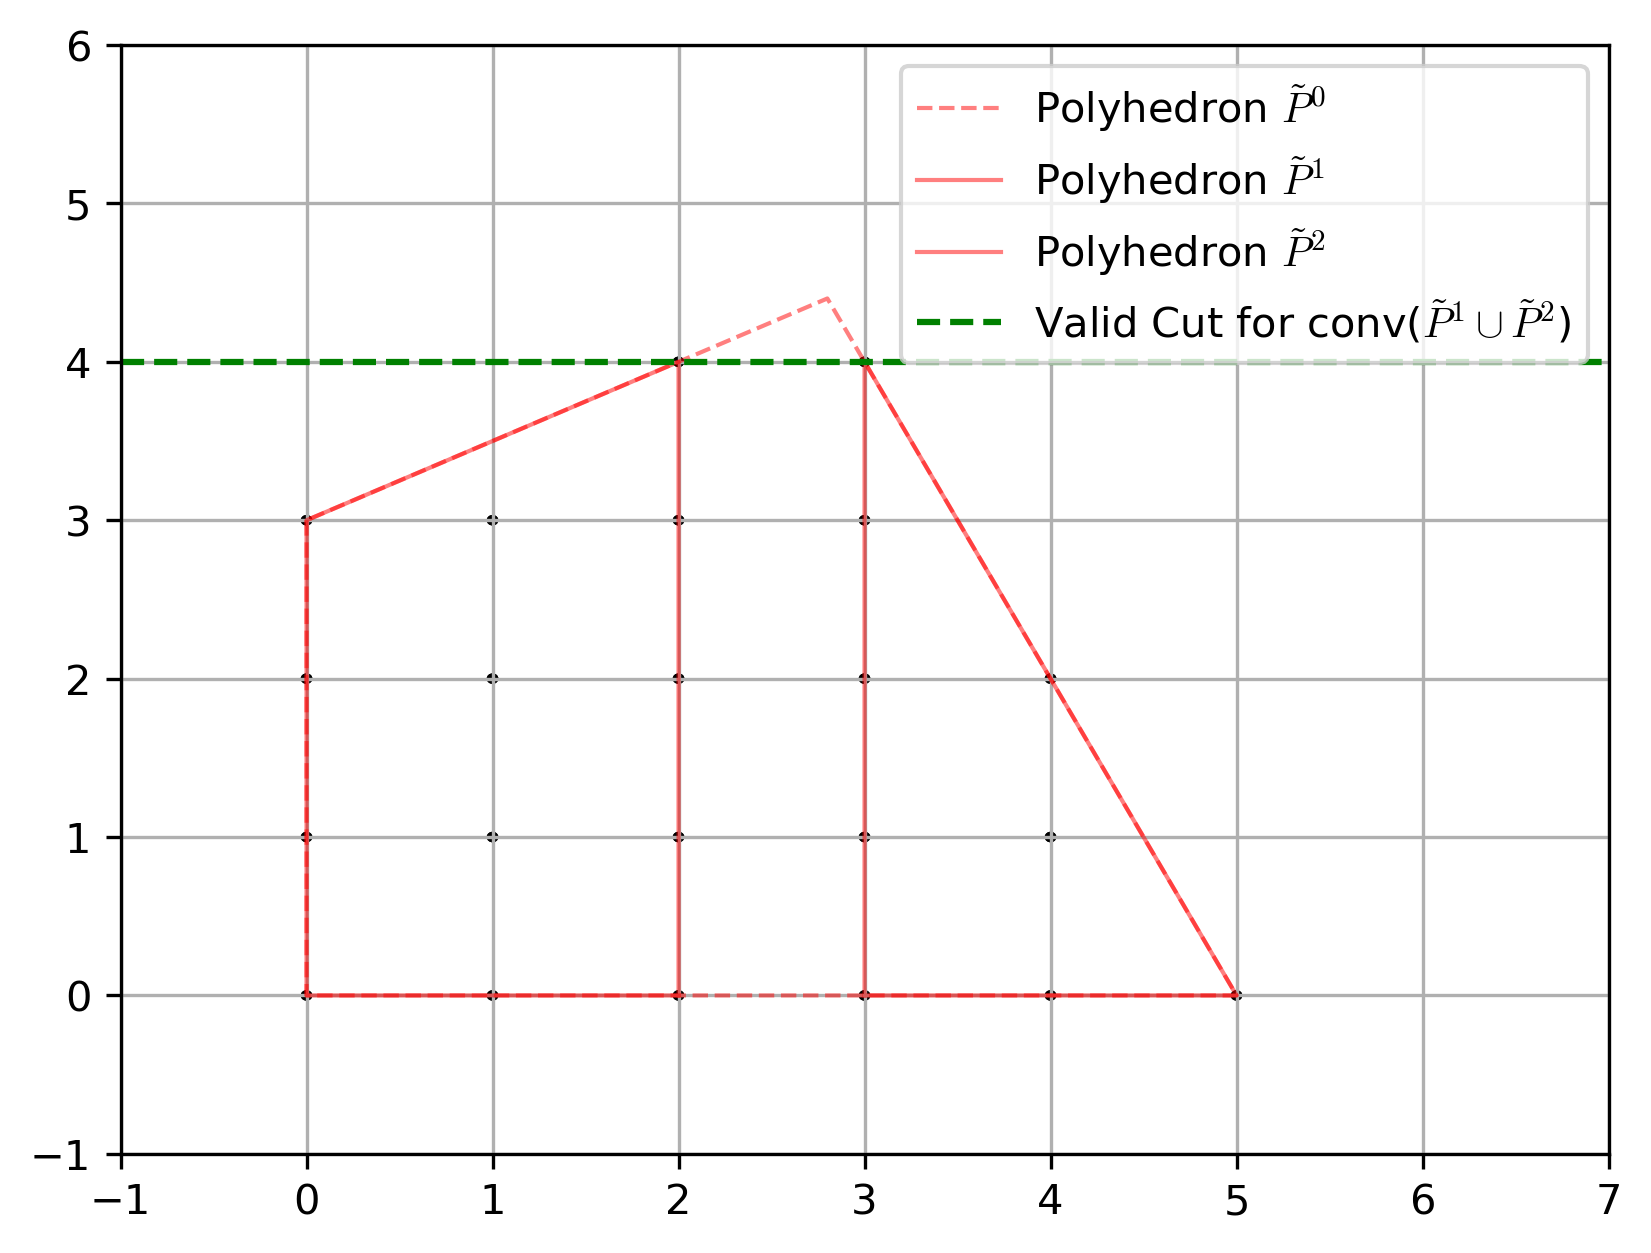
\includegraphics[]{PD_prime.png}
					}
					\caption{A cut valid for both of (\ref{right})'s subproblems}
					\label{p:hull}
				\end{figure}
			\end{column}
			\begin{column}{0.6\textwidth}
				\begin{itemize}
					\item We can achieve this goal by
					\begin{itemize}
						\item Tightening the root relaxation, $ \bar{P}^1 $, with cuts valid for all $ \bar{P}^t $ with $ t \in \mathcal{T}_1 $.
						\item Starting Branch and Bound with only the tightened $ \bar{P}^1 $ in the queue.
					\end{itemize}
					\item The above cuts are known as \textbf{Disjunctive cuts}.
					\item To find disjunctive cuts, we need
					\begin{itemize}
						\item A generator to create a disjunctive cut.
						\item A cut generation algorithm to run the generator.
					\end{itemize}
				\end{itemize}
			\end{column}
		\end{columns}
		\begin{block}{}
			We can create disjunctive cuts by implementing the Cut Generating LP (CGLP) and embedding it within a standard cut generation algorithm.
		\end{block}
		\normalsize
	\end{frame}

	\begin{frame}[t]
		\frametitle{Deriving Disjunctive Cuts}
		\small
		% with our tree defined, lets now define sufficient cuts
		\begin{itemize}
			% first two bullets just say a linear combo of constraints is itself a valid inequality
			\item Let $ \mu^{t} \in \Rmbb_+^m $, $ w^{t} \in \Rmbb_+^n $, $ v^{t} \in \Rmbb_+^n $, and $ I_n $ be the $ n $-dimensional identity matrix. 
			\item The following is valid for all $ x \in \bar{P}^{t} $:
			\begin{align}
				(A^T \mu^{t} + I_n w^{t} - I_n v^{t})x \geq {\mu^{t}}^T \bar{b}^{t} + {w^{t}}^T \ell^{t} - {v^{t}}^T u^{t} \label{e:valid_inequality}
			\end{align}
			% third bullet says to find an inequality valid for each of the linear combos 
			\item Let $ \pi \in \Rmbb^n $ and $ \pi_0 \in \Rmbb $ satisfy the following:
			\begin{align}
				\begin{split}
					\pi &\geq A^T \mu^{t} + I_n w^{t} - I_n v^{t} \\
					\pi_0 & \leq {\mu^{t}}^T \bar{b}^{t} + {w^{t}}^T \ell^{t} - {v^{t}}^T u^{t}
				\end{split} \; \text{ for all } t \in \mathcal{T}_1 \label{e:disjunctive_inequality}
			\end{align}
			% thus its valid for all terminal nodes of the MILP
			\item Since (\ref{e:valid_inequality}) is valid for all $ x \in \bar{P}^{t} $ and $ t \in \mathcal{T}_1 $, it follows $ (\pi, \pi_0) $ is a valid inequality for all $ \bar{P}^{t} $ with $ t \in \mathcal{T}_1 $.
			\vspace{.25cm}
			\begin{block}{}
				We conclude $ (\pi, \pi_0) $ is a disjunctive cut for (\ref{milpbar}).
			\end{block}
		\end{itemize}
		\normalsize
	\end{frame}

	\begin{frame}[t]
		\frametitle{Deriving the Cut Generating LP}
		\small
		\begin{itemize}
			% now that we know what makes a cut feasible, we can find the one that cuts off the estimate as much as possible
			\item We seek disjunctive cuts that tighten $ \bar{P}^1 $ as much as possible.
			\item Let $ x^* = \text{argmin}\{\bar{c}^T x : x \in \bar{P}^1 \} $.
			\item We define the CGLP given the set of nodes with indices in $ \mathcal{T}_1 $ as follows:
			\begin{equation} \tag{CGLP-$ \mathcal{T}_1 $}
				\begin{alignedat}{2} \label{e:cglp} 
					\text{maximize } \; \; \qquad & \pi_0 - \pi^T x^* && \\
					\text{subject to } \qquad \pi & \geq A^T \mu^{t} + I_n w^{t} - I_n v^{t} && \;  t \in \mathcal{T}_1 \\
					\pi_0 & \leq {\mu^{t}}^T \bar{b}^{t} + {w^{t}}^T \ell^{t} - {v^{t}}^T u^{t} && \; t \in \mathcal{T}_1 \\
					1 & = \sum_{t \in \mathcal{T}_0} \big( \sum_{j=1}^{m} \mu_j^{t} + \sum_{i=1}^{n} w_i^{t} + \sum_{i=1}^{n} v_i^{t} \big) && \\
					& \mu^{t} \in \Rmbb_+^{m}, \; w^{t} \in \Rmbb_+^n \; v^{t} \in \Rmbb_+^n && t \in \mathcal{T}_1
				\end{alignedat}
			\end{equation}
			\begin{block}{}
				We can solve CGLP-$ \mathcal{T}_1 $ repeatedly within a cutting plane algorithm to generate a set of increasingly tighter disjunctive cuts.
			\end{block}
		\end{itemize}
		\normalsize
	\end{frame}

	\begin{frame}[t]
		\frametitle{A Cutting Plane Algorithm Using the CGLP}
		\small
		\vspace{-.25cm}
		We can define a cutting plane algorithm to tighten $ \bar{P}^1 $ with disjunctive cuts valid for all $ \bar{P}^{t} $ with $ t \in \mathcal{T}_1 $ as follows: \\
		\vspace{.1cm}
		\textbf{Algorithm CPA-$ \bar{P}^1 $-$ \mathcal{T}_1 $}
		\begin{algorithmic}[1]
			\State $ \bar{P}^{1,0} := \bar{P}^1 $
			\State $ k := 0 $
			\While{True}:
			\State $ x^* = \text{argmin}\{\bar{c}^T x : x \in \bar{P}^{1,k} \} $
			\State Let $ (\pi^k, \pi^k_0) $ be the optimal solution to (\ref{e:cglp})
			\If{$ \pi^k_0 - {\pi^k}^T x^* \leq 0$}:
			\State \textbf{stop}
			\EndIf
			\State $ \bar{P}^{1,k+1} = \bar{P}^{1, k} \cap \{x \in \Rmbb^n: {\pi^k}^T x \geq \pi^k_0\} $
			\State $ k = k + 1$
			\EndWhile
			\State $ \bar{P}^1 = \bar{P}^{1,k} $
		\end{algorithmic}
		\vspace{-.1cm}
		\begin{block}{}
			We can warm start Branch and Bound for (\ref{milpbar}) by using the updated $ \bar{P}^1 $ as the root relaxation.
		\end{block}
		\normalsize
	\end{frame}

	\begin{frame}[t]
		\frametitle{Putting It All Together}
		\small
		% before going into how we find these cuts, we need to define how we update the tree off which we base them.
		We did the following to warm start solving (\ref{milpbar}) from the solve of (\ref{milp}):
		\begin{itemize}
			\item Apply the disjunction from (\ref{milp}) to (\ref{milpbar}), yielding
			\begin{itemize}
				\item A LP relaxation feasible region $ \bar{P}^t $ for all $ t \in B $
				\item A set of terminal nodes with indices $ \mathcal{T}_1 $
			\end{itemize}
			\item Formulate (\ref{e:cglp}) to find a cut valid for all $ \bar{P}^t $ with $ t \in \mathcal{T}_1 $.
			\item Run \textbf{CPA-$ \bar{P}^1 $-$ \mathcal{T}_1 $} to tighten $ \bar{P}^1 $.
			\item Solve (\ref{milpbar}) with Branch and Bound starting from the tightened $ \bar{P}^1 $.
		\end{itemize}
		\vspace{1.75cm}
		\begin{block}{}
			For this approach to be effective, \textbf{CPA-$ \bar{P}^1 $-$ \mathcal{T}_1 $} needs to run in less time than that saved from warm starting (\ref{milpbar})'s solve.
		\end{block}
		\normalsize
	\end{frame}
	
	\section{Computational Considerations}
	
	\begin{frame}[t]
		\frametitle{Handling Disjunctions with Many Terms}
		\small
		\begin{columns}[T]
			\begin{column}{0.5\textwidth}
				\begin{itemize}
					\item Consider the following branch and bound tree with terminal nodes $ \mathcal{T} = \{16, ..., 31\}$.
					\item CGLP-$ \mathcal{T} $ has $ |\mathcal{T}|m $ variables and $ |\mathcal{T}|(2n + m) $ constraints.
					\item Solving CGLP-$ \mathcal{T} $ can become intractible for MILPs where $ m $, $ n $ or $ |\mathcal{T}| $ is large.
				\end{itemize}
			\end{column}
			\begin{column}{0.5\textwidth}
				\vspace{.75cm}
				\begin{figure}[h]
					\resizebox{\textwidth}{!}{%
						\includegraphics[]{tree1.png}
					}
					\label{p:tree1}
				\end{figure}
			\end{column}
		\end{columns}
		\vspace{1.5cm}
		\begin{block}{}
			We need a way to decompose the CGLP into solvable subproblems that still yield cuts valid for the root node.
		\end{block}
		\normalsize
	\end{frame}

	\begin{frame}[t]
		\frametitle{Handling Disjunctions with Many Terms}
		\small
		\begin{columns}[T]
			\begin{column}{0.5\textwidth}
				Instead of running \textbf{CPA-$ \bar{P}^1 $-$ \mathcal{T}_1 $}, we can
				\begin{itemize}
					\item Run \textbf{CPA-$ \bar{P}^4 $-$ \textcolor{red}{\mathcal{T}^2_4} $}, \textbf{CPA-$ \bar{P}^5 $-$ \textcolor{yellow}{\mathcal{T}^2_5} $}, \textbf{CPA-$ \bar{P}^6 $-$ \textcolor{blue}{\mathcal{T}^2_6} $}, and \textbf{CPA-$ \bar{P}^7 $-$ \textcolor{violet}{\mathcal{T}^2_7} $}.
					\item Then run \textbf{CPA-$ \bar{P}^1 $-$ \mathcal{T}^2_1 $}.
				\end{itemize}
				The result of this is that
				\begin{itemize}
					\item More CGLPs will be solved.
					\item Each solved CGLP is significantly smaller.
				\end{itemize}
			\end{column}
			\begin{column}{0.5\textwidth}
				\vspace{-.25cm}
				\begin{figure}[h]
					\resizebox{\textwidth}{!}{%
						\includegraphics[]{tree2.png}
					}
					\label{p:tree2}
				\end{figure}
				Let $ \mathcal{T}^2_1 = \{4, ..., 7\} $, $ \textcolor{red}{\mathcal{T}^2_4} = \{16, ..., 19\} $, $ \textcolor{yellow}{\mathcal{T}^2_5} = \{20, ..., 23\} $, $ \textcolor{blue}{\mathcal{T}^2_6} = \{24, ..., 27\} $, and $ \textcolor{violet}{\mathcal{T}^2_7} = \{28, ..., 31\} $.
			\end{column}
		\end{columns}
		\vspace{1cm}
		\begin{block}{}
			We're exploring trade-offs between having fewer CGLP's to solve and solving smaller CGLP's to find the most effective way to refine the root node relaxation.
		\end{block}
		\normalsize
	\end{frame}

	\section{Open Source Contributions}
	% with what knowledge we can infer in hand, we now need to test our hypothesis
	
	\begin{frame}[t]
		\frametitle{Implementation Considerations}
		\vspace{-.25cm}
		\begin{columns}[T]
			\begin{column}{0.5\textwidth}
				\large
				\textbf{Goals}
				\small
				\begin{itemize}
					\item We need the following attributes to implement the CGLP:
					\begin{itemize}
						\item The branch and bound tree
						\item Each node's LP relaxation
					\end{itemize}
					\item We would like a Python implementation because Python
					\begin{itemize}
						\item Is quick to write
						\item Has a large community
					\end{itemize}
				\end{itemize}
			\end{column}
			\begin{column}{0.5\textwidth}
				\large
				\textbf{Limitations}
				\small
				\begin{itemize}
					\item No solver has a Python API with these attributes.
					\item Unsure of solver persisting these attributes.
				\end{itemize}
				\large
				\textbf{Solutions}
				\small
				\begin{itemize}
					\item Add these attributes to CBC/CyLP.
					\item Both are open source.
					\item CBC has the attributes, but they need persistence.
					\item CyLP converts CBC into Python.
				\end{itemize}
			\end{column}
		\end{columns}
		\small
		\begin{block}{}
			We can add to CyLP and persist in CBC the attributes we need for the CGLP to make them available in Python.
		\end{block}
		\normalsize
	\end{frame}

	\begin{frame}[t]
		\frametitle{CyLP Motivations}
		\small
		Because CyLP is a Cython package, its classes extend various classes of COIN-OR
		\begin{itemize}
			\item CyClpSimplex extends ClpSimplex.
			\item CyCbcModel extends CbcModel.
		\end{itemize}
		How Cython works:
		\begin{itemize}
			\item Python objects instantiate by binding a corresponding C/C++ instance.
			\item Function calls can call functions on the bound C/C++ instance.
			\item Attribute access can access attributes on the bound C/C++ instance.
			\item Any C/C++ code used by Python objects is compiled during packaging.
		\end{itemize}
		Advantages of using Cython:
		\begin{itemize}
			\item It makes existing C/C++ classes available in Python.
			\item It combines fast development of Python with fast execution of C/C++
		\end{itemize}
		\normalsize
	\end{frame}

	\begin{frame}[t]
		\frametitle{Introduction to Cython}
		\small
		Below is a typical example of how instantiation works in Cython:
		\begin{columns}[T]
			\begin{column}{0.5\textwidth}
				\begin{figure}[h]
					\resizebox{\textwidth}{!}{%
						\includegraphics[]{cyclp_init.png}
					}
					\caption{CyClpSimplex objects bind an instance of CppIClpSimplex to the \texttt{.cppSelf} attribute during initialization.}
					\label{p:cyclp_init}
				\end{figure}
			\end{column}
			\begin{column}{0.5\textwidth}
				\begin{figure}[h]
					\resizebox{\textwidth}{!}{%
						\includegraphics[]{iclp_init.png}
					}
					\caption{CppIClpSimplex is an alias for IClpSimplex, a subclass of ClpSimplex.}
					\label{p:iclp_init}
				\end{figure}
			\end{column}
		\end{columns}
		\normalsize
	\end{frame}

	\begin{frame}[t]
		\frametitle{Introduction to Cython}
		\small
		Below is a typical example of how function calls work in Cython:
		\begin{columns}[T]
			\begin{column}{0.65\textwidth}
				\begin{figure}[h]
					\resizebox{\textwidth}{!}{%
						\includegraphics[]{cyclp_readmps.png}
					}
					\caption{Reading a \texttt{.mps} file in CyLP}
					\label{p:cyclp_readmps}
				\end{figure}
			\end{column}
			\begin{column}{0.35\textwidth}
				\begin{itemize}
					\item CyClpSimplex reads \texttt{.mps} files by calling on ClpSimplex's eponymous function.
					\item Solving LP's with CyClpSimplex works analogously. 
				\end{itemize}
			\end{column}
		\end{columns}
		\normalsize
	\end{frame}

	\begin{frame}[t]
		\frametitle{Introduction to Cython}
		\small
		Below is a typical example of how attribute access works in Cython:
		\begin{columns}[T]
			\begin{column}{0.65\textwidth}
				\begin{figure}[h]
					\resizebox{.9\textwidth}{!}{%
						\includegraphics[]{cyclp_solution.png}
					}
					\caption{Accessing an LP primal solution in CyLP}
					\label{p:cyclp_solution}
				\end{figure}
			\end{column}
			\begin{column}{0.35\textwidth}
				\begin{itemize}
					\item CyClpSimplex's PrimalVariableSolution attribute returns the corresponding ClpSimplex attribute.
					\item Cython functions handle converting C/C++ types into Python types (e.g. \texttt{<object>} in line 302)
				\end{itemize}
			\end{column}
		\end{columns}
		\normalsize
	\end{frame}
	
	\section{Closing Thoughts}
	
	\begin{frame}[t]
		\frametitle{Putting It All Together}
		\small
		\begin{block}{}
			To recap, the CGLP generates cuts that retain primal and dual bounds from a MILP solve while resetting the underlying disjunction to a single node.
		\end{block}
		\begin{columns}[T]
			\begin{column}{0.5\textwidth}
				What we've accomplished:
				\begin{itemize}
					\item Implemented CGLP class in Python
					\item Developed algorithm to decompose CGLP for large disjunctions
					\item Added necessary branch and bound tree attributes to CyLP and CBC
				\end{itemize}
			\end{column}
			\begin{column}{0.45\textwidth}
				What's next:
				\begin{itemize}
					\item Integrate each accomplishment
					\item Test warm start effectiveness for MILP's with similar objectives or constraint bounds
					\item Further tune CGLP performance
					\item Test warm start effectiveness for MILP's with added variables or constraints
				\end{itemize}
			\end{column}
		\end{columns}
		\normalsize
	\end{frame}

	\section{Index}
	
	
	\begin{frame}[t]
		\frametitle{Numerical Experiments}
		\small
		\begin{columns}[T]
			\begin{column}{0.6\textwidth}
				\vspace{-.25cm}
				\begin{figure}[h]
					\resizebox{\textwidth}{!}{%
						\includegraphics[]{iterations_to_recover.png}
					}
					\label{p:iterations_to_recover}
				\end{figure}
			\end{column}
			\begin{column}{0.4\textwidth}
				\begin{itemize}
					\item We also need to consider how many iterations it takes a cutting plane algorithm to yield tight cuts.
					\item We see a linear relationship between disjunctive terms and number of cut generation iterations for each CGLP to recover the disjunction's dual bound.
				\end{itemize}
			\end{column}
		\end{columns}
		\vspace{.25cm}
		\begin{block}{}
			Knowing the convergence rate to a disjunction's dual bound for a cut generation algorithm using the CGLP may allow us to infer which size disjunctions to use.
		\end{block}
		\normalsize
	\end{frame}
	
	\begin{frame}[t]
		\frametitle{Numerical Experiments}
		\footnotesize
		\vspace{-.35cm}
		Cut generation algorithms using the CGLP to recover the dual bound for the given sized disjunctions below converge at similar rates.
		\vspace{-.1cm}
		\begin{figure}[h]
			\resizebox{.85\textwidth}{!}{%
				\includegraphics[]{disjunction_2.png}
			}
			\resizebox{.85\textwidth}{!}{%
				\includegraphics[]{disjunction_4.png}
			}
			\resizebox{.85\textwidth}{!}{%
				\includegraphics[]{disjunction_8.png}
			}
			\label{p:convergence}
		\end{figure}
		\vspace{-.25cm}
		\begin{block}{}
			No immediate advantages appear among different sized disjunctions and the number of cutting plane algorithm iterations required to derive tight cuts.
		\end{block}
		% just a relationship to keep in mind as we test trade offs between sizes of CGLP and number of them we solve
		\normalsize
	\end{frame}

	\begin{frame}[t]
		\frametitle{Restarting MILP's}
		\small
		\vspace{0cm}
		% thus concludes methodology, so let's talk applications
		\begin{itemize}
			\item Warm starting with a tightened root LP relaxation can be preferred to a partial tree already found on a looser root relaxation.
			\item We aim to identify problem classes where there is a strong preference for the former.
			\item When this is true, a partial solve followed by warm start method (c) takes less time than solving the instance cold.
			\item The idea then is as follows:
			\begin{itemize}
				\item Solve LP relaxations for certain number of nodes.
				\item Generate CGLP cuts against this tree.
				\item Tighten root node with these cuts.
				\item Restart Branch and Cut from beginning with tightened root relaxation.
			\end{itemize}
		\end{itemize}
		\vspace{0cm}
		\begin{block}{}
			If many problem classes exist where the above is beneficial, this would dramatically change how solvers work today.
		\end{block}
		\normalsize
	\end{frame}
	
	\begin{frame}[t]
		\frametitle{Branch and Price}
		\small
		\begin{itemize}
			\item We can tighten the LP relaxation for a MILP with the following formulation:
			\begin{align}
				\underset{x \in \text{conv}(\mathcal{S}_R)}{\text{ max }} \{c^T x | A''x \leq b''\}
				\intertext{where}
				\mathcal{S}_R = \{ x \in \Zmbb^n | A'x \leq b' \} \nonumber
			\end{align}
			\item With $ \mathcal{E} $ as the set of extreme points of $ \text{conv}(\mathcal{S}_R) $, we can reformulate as follows:
		\end{itemize}
		\begin{columns}
			\begin{column}{0.4\textwidth}
				\begin{equation}
					\begin{alignedat}{2}
						\text{max} \qquad \qquad & c^T x \\
						\text{s.t.} \quad \sum_{s \in \mathcal{E}} \lambda_s s & = x \\
						A'' x & \leq b'' \\
						\sum_{s \in \mathcal{E}} \lambda_s & = 1 \\
						\lambda & \in \Rmbb_+
					\end{alignedat} \nonumber
				\end{equation}
			\end{column}
			\begin{column}{0.05\textwidth}
				$ \implies $
			\end{column}
			\begin{column}{0.5\textwidth}
				\vspace{-.35cm}
				\begin{equation} \tag{DWLP}
					\begin{alignedat}{2}
						\text{max} \qquad  \sum_{s \in \mathcal{E}} \lambda_s(c^T &s) \\
						\text{s.t.}  \; \quad \sum_{s \in \mathcal{E}} \lambda_s (A''s) & \leq b'' \\
						\sum_{s \in \mathcal{E}} \lambda_s & = 1 \\
						\lambda & \in \Rmbb_+
					\end{alignedat}
				\end{equation}
			\end{column}
		\end{columns}
		\normalsize
	\end{frame}
	
	\begin{frame}[t]
		\frametitle{Branch and Price}
		\small
		\vspace{0cm}
		\begin{itemize}
			\item We solve (DWLP) by column generation, only ever using a subet of $ \mathcal{E} $. For dual values $ u $ and $ \alpha $ of (DWLP)'s constraints, we find a new $ s $ to augment the current subset by solving the following:
			\begin{align}
				-\alpha + \underset{x \in \mathcal{S}_R}{\text{max}} \{(c-uA'')x\} \label{LR} \tag{LR($ u $)}
			\end{align}
			\item (DWLP) is often the LP relaxation in Branch and Price. Notice (\ref{LR}) represents a series of closely related MILP's.
			\begin{itemize}
				\item Within a single solve of (DWLP), each (\ref{LR}) differs only by objective.
				\item A common branching technique in Branch and Price is to bound variables in (\ref{LR}). Thus, for fixed $ u $, (\ref{LR}) differs from its ancestor nodes by its RHS.
			\end{itemize}
		\end{itemize}
		\vspace{0cm}
		\begin{block}{}
			By warm starting the pricing problem in Branch and Price, we may be able to expand the sets of problems solved by this algorithm.
		\end{block}
		\normalsize
	\end{frame}
	
	\begin{frame}[t]
		\frametitle{Warm Starting Big Picture}
		\small
		\begin{block}{}
			We have a couple approaches at our disposal for warm starting a MILP from a previously solved one.
		\end{block}
		\begin{itemize}
			\item [(a)] Good warm start:
			\begin{itemize}
				\item Recalculate the primal bound.
				\item Restart Branch and Cut from the root node.
			\end{itemize}
			\item [(b)] Better warm start:
			\begin{itemize}
				\item Parameterize cuts.
				\item Recalculate the primal and/or dual bounds.
				\item Restart Branch and Cut from the leaf nodes.
			\end{itemize}
			\item [(c)] Hypothesized best warm start:
			\begin{itemize}
				\item Parameterize cuts.
				\item Add to the root relaxation cuts valid for all terminal subproblems.
				\item Restart Branch and Cut from the root node.
			\end{itemize}
		\end{itemize}
		\normalsize
	\end{frame}
	
	\begin{frame}[t]
		\frametitle{Next Steps}
		\small
		\begin{columns}[T]
			\begin{column}{0.45\textwidth}
				There are a few other problem classes we look to test the effectiveness of warm starts:
				\begin{itemize}
					\item Multiobjective MILP
					\item Primal Heuristics (RINS)
					\item Bilevel MILP
					\item Real-Time MILP
					\item MINLP
				\end{itemize}
			\end{column}
			\begin{column}{0.45\textwidth}
				We have the following next tasks in mind:
				\begin{itemize}
					\item Make cut generation numerically safe.
					\item Parametrize cut generation.
					\item Implement algorithms for each problem class.
					\item Run experiments for each algorithm comparing warm started version to current algorithms.
				\end{itemize}
			\end{column}
		\end{columns}
		\begin{block}{}
			We intend to test our warm starting methods against the problem classes mentioned in this presention to determine which can leverage these approaches to more effeciently be solved.
		\end{block}
		\normalsize
	\end{frame}

	\begin{frame}[t]
		\frametitle{Simple Approach to Warm Starting}
		\small
		\begin{itemize}
			\item Warm starting means to reuse a Branch and Bound tree from solving a previous MILP when solving a new one.
			\item One approach is to reevaluate leaf nodes' solutions at the new MILP’s objective and RHS to set applicable bounds. Then leaf nodes are placed into a priority queue, and Branch and Cut resumes.
			\item This approach has the following advantages:
			\begin{itemize}
				\item [(a)] When only the objective changes, all previously feasible solutions remain feasible. We can start the primal bound as the one with the best evaluation of the new objective.
				\item [(b)] When only the RHS changes, each node's dual LP relaxation maintains the same feasible region. We can start the dual bound of each node as its previous dual LP solution evaluated at the new RHS.
				\item [(c)] Restarting from the leaf nodes prevents us from having to branch and bound to regenerate them in the new instance.
			\end{itemize}
		\end{itemize}
		\normalsize
	\end{frame}

	\begin{frame}[t]
		\frametitle{Simple Approach to Warm Starting}
		\small
		\begin{itemize}
			\item Warm starting means to reuse a Branch and Bound tree from solving a previous MILP when solving a new one.
			\item One approach is to reevaluate leaf nodes' solutions at the new MILP’s objective and RHS to set applicable bounds. Then leaf nodes are placed into a priority queue, and Branch and Cut resumes.
			\item This approach has the following disadvantages:
			\begin{itemize}
				\item [(a)] The primal or dual bound is weak if the objective or RHS changes significantly.
				\item [(b)] Potentially many leaf nodes will need to be branched.
				\item [(c)] Generated cuts may no longer be valid if RHS changed.
			\end{itemize}
		\end{itemize}
		\vspace{.5cm}
		\begin{block}{}
			Starting a MILP solve with a Branch and Bound tree from a previous solve can be a simple and quick way to improve performance, but such an approach is not a panacea.
		\end{block}
		\normalsize
	\end{frame}

	\begin{frame}[t]
		\frametitle{Motivating the Cut Generating LP}
		\small
		\begin{itemize}
			\item Generating strong cuts of the convex hull of the previous disjunctive terms’ LP relaxations near the new optimal solution ameliorates disadvantages (a) and (b). Instead of reusing the previous tree to solve our problem, we solve with a new Branch and Bound tree with these cuts added to the root LP relaxation.
			\item This removes advantages (b) and (c) but tightens the root LP relaxation. In many cases this is preferred because it can more quickly give the solver an idea of where to search for an optimal solution.
			\item These cuts are the valid inequalities that violate by as much as possible our best estimates of the new optimal solution.
			\item Given such estimates, the Cut Generating LP (CGLP) finds such inequalities.
		\end{itemize}
		\vspace{.25cm}
		\begin{block}{}
			It may be possible to improve a warm start by replacing the previous tree with strategically chosen strong cuts of the convex hull of its disjunctive terms' LP relaxations.
		\end{block}
		\normalsize
	\end{frame}

	\begin{frame}[t]
		\frametitle{Handling Constraint Bound Changes}
		\small
		\vspace{-.25cm}
		\begin{itemize}
			\item Should $ b^k \neq b^{k'} $, $ (A^{kt}, b^{kt}) $ may no longer be valid for the matching disjunctive term in MILP $ k' $. Thus, MILP $ k $'s tree may not be able to warm start MILP $ k' $.
			
			\item Let $ p_{k't}(A^{kt}, b^{kt}) = (p_{k't}(A, b^k), p_{k't}(\Pi^{kt}, \Pi_0^{kt})) : \Rmbb^{m^t \times n + 1} \rightarrow \Rmbb^{m^t \times n + 1} $ map the constraints $ (A^{kt}, b^{kt}) $ to constraints that are valid for matching disjunctive term in MILP $ k' $, where
			\begin{itemize}
				\item $ p_{k't}(A, b^k) = (A, b^{k'}) $
				\item $ p_{k't}(\Pi^{kt}, \Pi_0^{kt}) $ updates each GMI cut as described in Guzelsoy (2006) and each CGLP cut $ (\pi, \pi_0) $ as follows. Let the tree of MILP $ \kappa $ be from which $ (\pi, \pi_0) $ is derived. Let $ (\tilde{A}, \tilde{b}) = p_{k't}(A^{\kappa t}, b^{\kappa t}) $. Then
				\begin{align*}
					(\pi, \pi_0) =& (\text{max} \{\tilde{A}^T \mu^{kt} + {I_n}^T w^{kt} - {I_n}^T v^{kt} \; \text{ for all } t \in \mathcal{T}^k\}, \\
					& \qquad \text{min} \{\tilde{b}^T \mu^{kt} + {l^{kt}}^T w^{kt} - {u^{kt}}^T v^{kt} \; \text{ for all } t \in \mathcal{T}^k\})
				\end{align*}
			\end{itemize}
		\end{itemize}
		\vspace{-.25cm}
		\begin{block}{}
			If $ b^k \neq b^{k'} $, cuts generated for MILP $ k $ must be made valid for MILP $ k' $ before the tree of MILP $ k $ can be used to warm start MILP $ k' $.
		\end{block}
		\normalsize
	\end{frame}
	
	\begin{frame}[t]
		\frametitle{Warm Starting Big Picture}
		\small
		\vspace{-.5cm}
		\begin{itemize}
			\item There are a couple of different approaches we can take to warm starting a MILP $ k' $ from one previously solved, MILP $ k $.
			\item All look to accomplish the same thing, but they differ from each other in the following ways:
			\begin{itemize}
				\item When solving MILP $ k' $ with the tree from MILP $ k $'s solve and only the objectives differ between the two instances, there is no need to transform cuts, and only the feasible leaves need searched. However, the dual function is lost, so search priority is less clear.
				\item When solving MILP $ k' $ with the tree from MILP $ k $'s solve and only the RHS's differ between the two instances, cuts may need to be transformed to remain valid, and all leaves need searched. However, the dual function remains intact, so search priority is clearer.
				\item When generating CGLP cuts from MILP $ k $ to warm start MILP $ k' $, a partially searched tree is exchanged for a tighter root relaxation. Some nodes may be re-evaluated, but the number of nodes to search may be reduced.
			\end{itemize}
		\end{itemize}
		\normalsize
	\end{frame}

		\begin{frame}[t]
		\frametitle{Dual Decomposition for Stochastic MILP}
		\small
		\vspace{-.25cm}
		% for a more practical example, we're also looking at warm starting decomposable MILP's like
		\begin{itemize}
			\item Let $ S^j := \{(x, y^j): Ax \leq b, x \in X, T^j x + w y^j \leq h^j, y^j \in Y\} $
			\item A multistage stochastic MILP can be formulated as follows:
			% the deterministic formulation
			\begin{align}
				\text{max} \left\{ c^T x + \sum_{j=1}^{r} p^j {q^j}^T y^j : (x, y^j) \in S^j \text{ for } j \in [r] \right\} \label{smilp1}
			\end{align}
			\item It can be reformulated as follows:
			% make scenarios independent but tie them together with linking constraints
			\begin{align}
				\text{max} \left\{ \sum_{j=1}^{r} p^j (c^T x^j + {q^j}^T y^j) : (x^j, y^j) \in S^j \text{ for } j \in [r], x^1 = ... = x^r \right\} \label{smilp2}
			\end{align}
			\item For $ H^j $ such that $ \sum_{j=1}^{r} H^j x^j = 0 $ is equivalent to $ x_1 = ... = x_r $, (\ref{smilp1}) and (\ref{smilp2}) can have an upper bound decomposed as follows:
			% for sufficiently structured H, we can minimize its product with x, remove it from the constraints, and get the following upper bound
			\begin{align}
				& \qquad \qquad \qquad \qquad \qquad \underset{\lambda}{\text{ min }} D(\lambda) \label{LD} \tag{LD} \\
				D(\lambda) &= \text{max} \left\{ \sum_{j=1}^{r} p^j (c^T x^j + {q^j}^T y^j) + \lambda(H^j x^j) : (x^j, y^j) \in S^j \text{ for } j \in [r] \right\} \nonumber
			\end{align}
		\end{itemize}
		\normalsize
	\end{frame}
	
	\begin{frame}[t]
		\frametitle{Dual Decomposition for Stochastic MILP}
		\small
		\vspace{0cm}
		% when we look at how we solve (LD), we see a lot of opportunity to warm start
		\begin{itemize}
			% the solve method is
			\item $ D(\lambda) $ consists of $ r $ independent MILP's.
			\item (LD) is solved by a subgradient algorithm. We branch on the average value of $ x $ in (LD)'s solution and bound (LD) again until $ x^j $ are all identical.
			% the opportunities for warm starting are
			\item Notice there are $ r $ series of MILPs sharing similar structure:
			\begin{itemize}
				\item MILP $ j $ in $ D(\lambda) $ differs from MILP $ j $ in $ D(\lambda') $ only by objective.
				\item MILP $ j $ in $ D(\lambda) $ before branching differs from MILP $ j $ in $ D(\lambda) $ after branching only by variable bounds.
			\end{itemize}
		\end{itemize}
		\vspace{1.5cm}
		\begin{block}{}
			Since solving a multistage Stochastic MILP involves solving multiple series of potentially difficult MILPs, the warm starting techniques presented earlier could be beneficial to the solution method.
		\end{block}
		\normalsize
	\end{frame}
	
\end{document}
